\chapter{Conclusion and Further Research}
\label{ch:conc}
To conclude an answer to the initial research question is given, and the results are discussed. An improved reactive concession strategy is given, and to finalize further research options are shown. 
\section{Conclusion}
In this thesis an overview of agent solutions used in the manufacturing world is given. It is found that a gap lies in the ``real'' negotiation, which excludes the use of auctions and the contract net protocol. By using the alternating offer protocol, it is checked whether an optimal solution can be found. At the moment, it seems as if the reactive concession strategy, as described in \citet{zheng2015automated} still has some difficulties. This can be clearly seen in \Cref{fig:reactivevsnon-reactive}. 

So although the reactive concession strategy ensures that the agents only concede when the other agents concede, it under-performs. However, when looking at the individual utility of an agent, it might be the best protocol to implement since it ensures that an agent only concedes if the other agents do as well.

The usage of private utility functions allows for competing companies to use automated negotiation. This is in line with the idea of Industry 4.0, where companies specialize, but require products from other producers. By implementing automated negotiation, without the requirement of releasing the utility functions, competing businesses can flourish together. This conform to the principled negotiation ideology, which allows an optimal outcome.

So, how can energy and manufacturing companies use the AI concept of intelligent multi-agent systems (MAS) for the optimization of production process? Most importantly is that the production is shifting towards a decentralized control system. As discussed, the complexity of the system increases enormously. This means that the different nodes of the system have to communicate, while the notes might have conflicting ideas and (sub-) solutions. Using negotiation these conflicts can be solved. 

The optimal framework, using the sequential projection method with a monotonic concession protocol, allows for a system to find a solution, as shown with the use case.

From here on more domains can use negotiation, not only in the manufacturing. An example is the interaction between pedestrians, cars, public transport at an interjection when most of these get automated. Who gets the right of way when most central control structures, like the traffic lights, might disappear? Future asks for automatic negotiation.

\section{Discussion}
Although the alternating offer protocol has been used, it is not usable at all yet in a real case. The largest difficulty lies in the realistic portrayal of the utility function. The requirement for a convex utility function makes it even more difficult. However, if only the non-reactive strategy was used, it should be possible to use a non-convex function.

In the literature the concept of principled negotiation is discussed. Addressed is the importance of retaining a private utility function, but making it very important to create these utility functions to ensure objective negotiation. This we have achieved, and thus we can say that the negotiation in this thesis is a form of principled negotiation.

In the problem statement, the option of optimizing a production process using negotiation is discussed. It can be concluded that this has not fully been achieved. However, when looked at the implementation of multilateral multi-issue negotiation, without a mediator, and using a very simplified theoretical solution, this is achieved. 

Originally the preferred reference would have been to use the real data to compare this to the use case's current performance. This was not conceivable unfortunately due to the complexity of the system. Instead of using the Key Performance Indicator (KPI) of the business, an theoretical situation was checked. 

The use case was not an entirely optimal situation for the research. It had all the requirements for a multilateral multi-issue negotiation, but the fact that the agents had no purpose to keep their utility private was not a requirement. This addition would have had more impact when looking at processes that require privacy.

\subsection{Discussion of the Reactive Concession Strategy}

A difficulty is that no concession is seen if an agent concedes in a matter that the other agents have no desire in. So if, for example, the Anion concedes in the amount of water to produce (which means that it will produce more water), this concession will not be ``seen'' by the Neut, since it has no desire in this utility. 

Even worse is the opposite, an agent can perceive that an agent wants an higher utility than initially. %A large flaw in the reactive concession strategy is that an agent can simply propose new offers on its utility curve without making a concession. The other agent can see this as a concession and make a concession. This results in uneven distributed concessions made. 

Take for example the Anion and Neut from the use case. When the Neut looks at the concessions that the Anion does, he perceives an ``anti-concession'', since the Anion increases the Acid in the offer. 

In the beginning the Anion proposes 0 acid and 1 base. In the first round the Anion already proposes 0.5 acid. Since it takes the average of all acid proposals (both the Mixbed and Cation start with 1 acid), the weight of the Acid proposal is 0.5. This is the value that the Anion will propose, and the Neut perceives a decrease in the offer made by the Anion. This while the Anion actually does concede by increasing the water offer and decreasing the base.

A possible solution is as follows:
Since an agent's offer is equal to the weight of the proposals for issues it is indifferent about, the other agents can check. The agent knows the weight of the proposals and the offer of the agent. If the offer is equal to the weight for an issue, the proposal will be equal to the offer. This means that the agent that has proposed is indifferent for an issue. 

There are two situations where the proposal is equal to the weight for an issue. Either the agent is indifferent for that issue, and does not project it onto its indifference curve, or the weight is above the agents' indifference curve. Meaning that an agreement to the proposal is made.

If an agent is indifferent to the issue, the other agent must ignore the proposal the agent has done on the issue when looking at the concession. This can be done be setting the proposed value to the agents proposal at initiation.

From this it is possible to update the reactive concession strategy as shown in \Cref{al:algorithm2}. For clarification, we notate an issue $l$ within $x$ as $a_l\in x$ instead of the notation $x_j \in x$ as described in \Cref{sec:design:negmod}. An attempt to keep the algorithm as similar as possible to the original is attempted, since converge was already proven.

The weight is commonly known, since it is the average of all proposals, and thus the average value of each issue is also known. This is notated as $w_l \in w_t$.  
 
\begin{algorithm}[h]
$\Delta u_{j0} = s^0_j(t)-s^0_j(t-1)$\nllabel{al:start2}\;
\ForEach{$k\in {1,2,3,4}$}
{
	\eIf{$u_j(x^k_t) \geq ru_j$  \nllabel{al:nonreactive2}}{
		$\Delta u_{jk} \leftarrow \Delta u_{j0}(t) $\;
	}{
		\ForEach{$a_l \in x^k_t$}{
			\eIf{$a_l == w_l$}{
				Issue is indifferent for agent $k$\;
				Set to agent's initial value\;
				$z^k_l  =  x^k_0$\;
			}{
				Issue is important for agent $k$\;
				$z^k_l = x^k_t$\;
			}
		}
		$\Delta_1 u_{jk}(t) \leftarrow u_j(z^k)-u_j(x^k_{[j,-1]})$\;
		$\Delta_2 u_{jk}(t) \leftarrow u_j(z^k)-u_j(x^k_0)-(1-u_j(x^j_{t-1}))$\;
		$\Delta u_{jk} \leftarrow \max \{\Delta_1u_{jk}(t), \Delta_2u_{j
			k}(t),0\}$\;
	}
	$\Delta u_j(t)\leftarrow \min \{\displaystyle \min_{k\in 1, 2, 3, 4}\Delta u_{jk}(t), \Delta u_{j0}(t)\}$ \nllabel{al:end2}\;	
}
Agent $i$ concedes by determining $s_i(t)\leftarrow s_i(t-1)-\Delta u_j(t)$\;
\caption{Updated reactive concession strategy of \Cref{al:algorithm1} on \cpageref{al:algorithm1}. By checking whether the issue is indifferent for the agent, the appropiate concession is seen.}
\label{al:algorithm2}
\end{algorithm}
\clearpage
\section{Further Research}
As discussed, more research has to be conducted before negotiation can commonly be used in production and manufacturing. Some further research subjects are discussed here. Especially a lot of further research could be done on the alternating offer protocol to be able to use this method in manufacturing by looking at more concession strategies for example. Another option is that the agents could be improved to allow reasoning, using a holonic structure for example. Furthermore, other strategies can be used, while the utility functions can be changed as well. Also possible is the implementation of coalitions. Extra negotiation could be applied using bilateral negotiations, and to finalize heuristic learning methods can be applied.

\subsection{Extra concession strategies}
The many concession strategies, as shown in \Cref{sec:concessionstrat} allow for other strategies to be used. Further research could include using the utilities as described in that section, and compared to each other. Especially the \textit{fraction of utility} method should be considered, which was suggested as another good solution by \citet{wu2009efficient}. 

\subsection{Holonic Agents}
The structure of a holonic agent is that of a holon as can be seen in \Cref{fig:holonexample}. As shown in the literature (\Cref{ch:literature}), it is based on PROSA by \citep{van1998reference}. Ideally this could be implemented in this use case to make use of the different parts of the anion filter.
\begin{figure}[h]
	\centering
	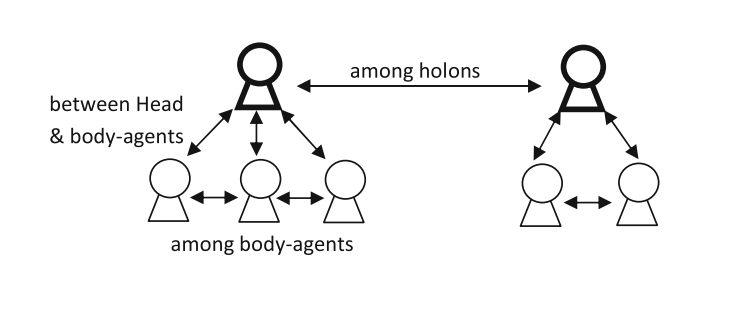
\includegraphics[width=0.7\linewidth]{img/holon_example}
	\caption{An example of the different negotiation between holons from \citet{beheshti2016negotiations}.}
	\label{fig:holonexample}
\end{figure}

The sub-agents of the Anion would consist of the different filters, as where originally shown in \Cref{sec:demi}. A consequence of the simplification made in this research, is that an assumption is made that the Anion can clean (receive base) and produce (make water) at the same time. This however is not always possible, since this depends on the current state of the filter. 
\begin{figure}[h]
	
	\centering
	\begin{tikzpicture}
	
	\node[circle,draw,  minimum size=1cm] (A1) at  (0,0) {A$_1$};
	\node[circle,draw,  minimum size=1cm] (A2) at  (0,-1.5) {A$_2$};
	\node[circle,draw,  minimum size=1cm] (A3) at  (0,-3) {A$_3$};
	\node[circle,draw,  minimum size=1cm] (A4) at  (0,-4.5) {A$_4$};
	\node[circle,draw,  minimum size=1cm] (A5) at  (0,-6) {A$_5$};
	\node[circle,draw,  minimum size=1cm] (A6) at  (0,-7.5) {A$_6$};
	%\draw  (0,-2.5) ellipse (1 and 3.4);
	
	\node[ellipse,  draw, minimum height =9cm, minimum width = 2.5cm ] (A) at (0,-3.75) {Anion};
	
	\end{tikzpicture}
	\caption{Anion head and sub-agents}
	\label{fig:anion-head-sub}
	
\end{figure}

The following facts and rules would then be part of the Anion, meaning that a beginning towards a representation of Beliefs, desires, and intentions, (BDI) in the agent can be made \citep{rao1995bdi}.

\begin{enumerate}
	\item
	Knowledge of anion head about the sub-agents:
	\begin{itemize}
		\item {$\{A_1, ..., A_6\}$ can process $a$ amount of water}
		\item {$\{A_1, ..., A_6\}$ needs to be cleaned after $b$ water}
		\item {$\{A_1, ..., A_6\}$ has filtered $c$ amount of water}
		\item {$\{A_1, ..., A_6\}$ needs $d$ base to clean}
		\item {$\{A_1, ..., A_6\}$ needs $e$ time to clean}
	\end{itemize}
	\item
	Currently $x$ amount of water being filtered 
	\item
	Currently $Z \subseteq \{A_1, ..., A_6\}$ filter being used for water filtering
	\item
	Currently $Y \subseteq \{A_1, ..., A_6\}$ filter being used for cleaning
	\item
	Currently $w$ amount of base being used for cleaning
\end{enumerate}

The use of these holons would allow an agent to reason about the environment, and act upon it accordingly.

\subsection{Collaboration }
Not used and discussed, but an interesting research is the collaboration between agents which share a common interest. For example the Anion and Cation could collaborate against the Mixbed, since they both have no interest in producing water. By combining collaboration with the learning methods it could be possible to learn who shares the same desires.

\subsection{Utility function}
The requirement of a convex function forced the use of a specific and highly theoretical function. This could be perfected using more expert input. Although an attempt was made, using a variable in the Mixbed ratio, this of course still is a highly theoretical and unrealistic representation.
\subsubsection{Reservation curve}
A linear reservation curve was used for simplicity, since this eliminated the minimization (mixed integer programming) that would have been necessary if a truly curved function was used. An example is shown in \Cref{fig:anionreservationfunction}. The downside of this reservation curve is that the projection method would be a minimization problem, which is computationally heavy. 
\begin{figure}[h]
	\centering
	\begin{tikzpicture}[domain=0.15:4]
	%\draw[very thin,color=gray] (0.01,0.01) grid (3.9,3.9);
	\draw[->] (0.02,0) -- (4.2,0) node[below] {$Water$};
	\draw[->] (0,0.02) -- (0,4.2) node[left] {$Base$};% node[pos=0.25, left] {$200 m^3 / hr$};
	\draw[color=black] plot (\x,{0.07*exp(\x)}) node[left] {$R_A$};
	\end{tikzpicture}
	\label{fig:anionreservationfunction}
	\caption{A more realistic reservation curve for the Anion filter: if more water is filtered and given, the more base it requires.}
\end{figure}
\subsubsection{Learning methods}
As shown in \Cref{neg:learn}, learning methods can also be used to learn the desired utility function. This has not been done since the requirement of a convex utility function forced the usage of predefined functions.

It would be very interesting to see how learning could be implemented in combination with the reactive concession strategy. Would there still be an incentive to concede if the agents learn that if other agents concede they can obtain their optimum? Or do the agents learn that without concession, no solution is found?

\subsection{Continue negotiation after group agreement}
After the group has an agreement, the agents now allocate the resource as predefined (see \Cref{sec:design:mean}). This could be optimized to bilateral negotiation between the agents. Take the Mixbed and Anion for example: if the group agrees to an allocation of 0.5 base, the Mixbed and anion can further negotiate how much of this 0.5 should be allocated to whom. This new bilateral negotiation is simpler, and due to the fact that it only contains a single issue, allows for quick determination.
\nocite{baarslag2013evaluating}